\documentclass{standalone}
\usepackage{tikz}
\usepackage{ctex,siunitx}
\setCJKmainfont{Noto Serif CJK SC}
\usepackage{tkz-euclide}
\usepackage{amsmath}
\usetikzlibrary{patterns, calc,3d}
\usetikzlibrary {decorations.pathmorphing,decorations.pathreplacing,decorations.shapes}
\begin{document}
\small
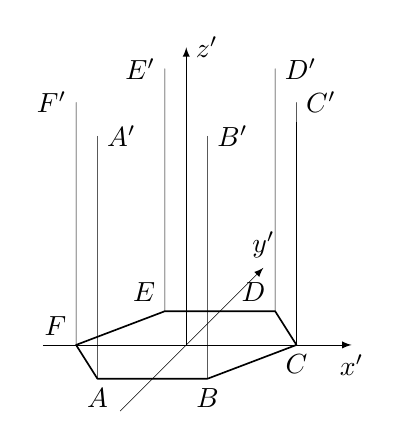
\begin{tikzpicture}[>=latex,scale=1.4]
  \tkzDefPoints{0/0/O',-1/0/F,1/0/C,-0.8062/-0.3062/A,0.1938/-0.3062/B,0.8062/0.3062/D,-0.1938/0.3062/E,0/2.2/O}
  \draw[very thin,->](-1.3,0)--(1.5,0)node[below]{$x'$};
  \draw[very thin,->](-0.6,-0.6)--(0.7,0.7)node[above]{$y'$};
  \draw[very thin,->](0,0)--(0,2.7)node[right]{$z'$};
  \tkzDefPointsBy[translation=from O' to O](A,B,C,D,E,F){A',B',C',D',E',F'}
  \tkzDrawPolygon[semithick](A,B,C,D,E,F)
  \tkzDrawSegments(A,A' B,B' C,C' D,D' E,E' F,F')
  \tkzLabelPoints(A,B,C)
  \tkzLabelPoints[above left](F,E,D)
  \tkzLabelPoints[left](F',E')
  \tkzLabelPoints[right](A',B',C',D')
\end{tikzpicture}
\end{document}